% !TEX TS-program = xelatex
% !TEX encoding = UTF-8 Unicode
% !Mode:: "TeX:UTF-8"
\documentclass[14pt]{resume}
\usepackage{graphicx}
\usepackage{tabu}
\usepackage{multirow}
\usepackage{multicol}
\usepackage{progressbar}
\usepackage{zh_CN-Adobefonts_external}
\usepackage{linespacing_fix}
\usepackage{cite}

\begin{document}
\pagenumbering{gobble}

\begin{multicols}{4}
    \Large{
        \begin{tabu}{ r }
            \multirow{5}{1in}{
                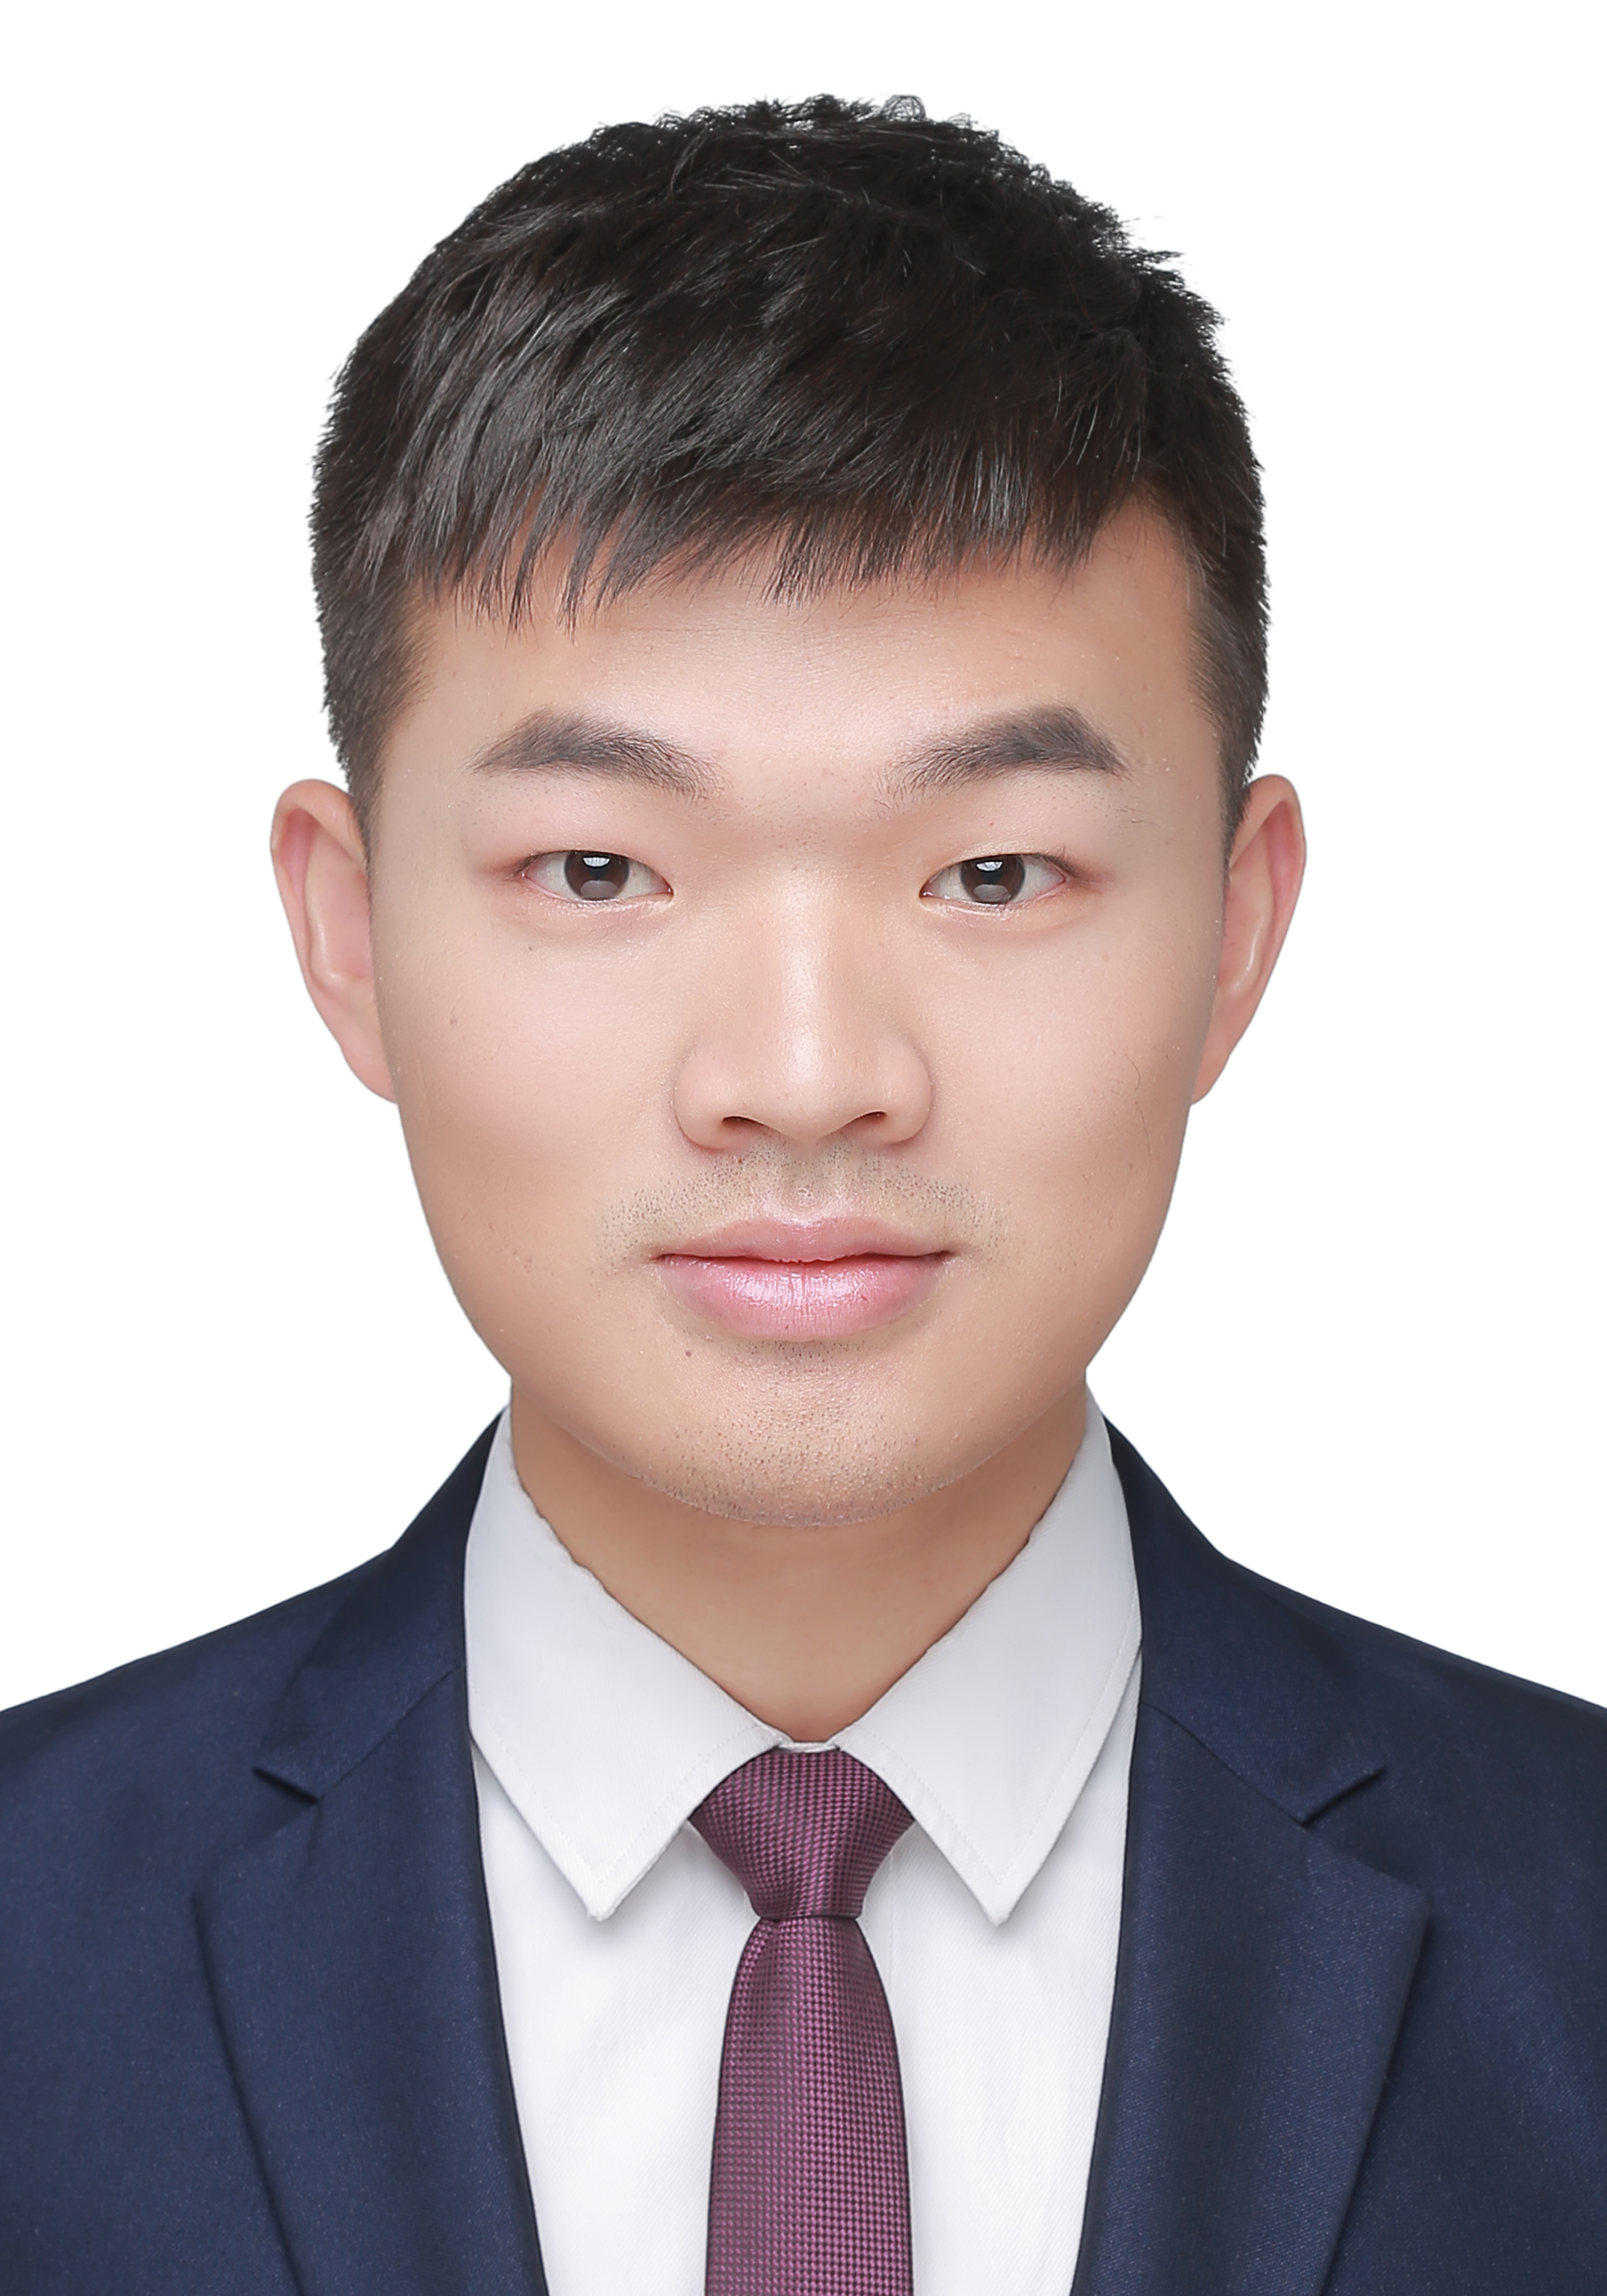
\includegraphics[width=0.88in]{avatar}
            }
        \end{tabu}
    }
    \columnbreak
    \Large{
        \begin{tabu}{ l l }
            & \faBirthdayCake{1995.09.12} \\
            & \phone{(+86)17600535912} \\
            & \email{izhouwl@163.com} \\
            & \homepage[www.zhouweilin.cn]{https://zhouweilin.cn} \\
            & \github[github.com/Si3ver]{https://github.com/Si3ver} 
        \end{tabu}
    }
    \columnbreak
    \Large{
        \begin{tabu}{ r }
            \multirow{5}{3.5in}{
                \name{周伟林}
                \basicInfo{
                    \faSmileO{意向职位:web前端研发}
                }
            }
        \end{tabu}
    }
\end{multicols}

% 教育背景
\section{\faGraduationCap\  教育背景}
\datedsubsection{\textbf{北京邮电大学(硕士)\quad\quad\quad}{ 网络技术研究院 \quad\quad\quad }{ 计算机科学与技术 }}{2016.09 - 2019.06}
\datedsubsection{\textbf{北京工业大学(本科)\quad\quad\quad}{ 计算机学院     \quad\quad\quad\quad\quad}{ 信息安全 }}{2012.09 - 2016.06}

% 技能树
\section{\faCogs\ 技能树}

\begin{itemize}
    \item[\faTree] 熟悉HTML、CSS、JavaScript,数据结构与算法
    \item[\faTree] 熟悉前端框架Vue,有mpVue开发电商小程序的经验
    \item[\faTree] 熟悉git原理及多人协作开发方式,了解简单的webpack配置
    \item[\faTree] 熟悉python、nodejs,了解中间件koa、mySQL数据库、Docker、k8s等后台技术
    \item[\faTree] 熟悉计算机网络、通信协议、信息安全等基础知识
    \item[\faTree] 了解数据可视化,熟悉EChart库的使用,会使用Matplotlib、LaTex\footnote{本简历使用LaTex书写并编译} 
    \item[\faTree] 无障碍阅读英文文档(CET-6),熟练使用Google、Stack Overflow检索
\end{itemize}

% 实习经历
\section{\faBriefcase\ 实习经历}

\datedsubsection{\textbf{北京美到家科技\quad\quad} \textbf{产品技术部\quad\quad\quad\quad}{ WEB前端研发}}{2018.11 - 如今}
\begin{itemize}
    \item[\faFlagO] 用Vue.js独立开发公司新主页,使用了MuseUI和Vue.js与王亮一起开发魔镜BA页,参与珠宝电商平台微信小程序的用户信息部分。
    \item[\faFlagO] 微信小程序使用mpVue框架开发,UI讨论出设计图后,后端定义数据库字段和表后,由前端负责在easy mock上定义接口格式,再交由后端实现和反馈。
    \item[\faCode] 本人独立负责用户中心的九个页面开发,包括路由和页面间参数传递。 
    \item[\faCheck] 小公司扁平化管理,获得与CEO、公司技术合伙人直接接触交流的机会。
\end{itemize}


\datedsubsection{\textbf{滴滴出行\quad\quad\quad\quad\quad} \textbf{质量技术部\quad\quad\quad\quad}{ WEB前端研发}}{2018.05 - 09}
\begin{itemize}
    \item[\faFlagO] 参与了Omega项目的前端页面开发工作,包括编写客服反馈、安卓错误上报等页面。
    \item[\faCode] 使用自制模板引擎simplite与原生JS开发,并使用node打包编译上线。
    \item[\faCheck] 熟悉了模板引擎开发的方式和Echarts库的使用。
    \item[\faCheck] 经测试、产品检验和反馈,页面上线到正式系统中,供公司内部使用。 
\end{itemize}

\datedsubsection{\textbf{西门子中国\quad\quad\quad\quad} \textbf{新闻传播部\quad\quad\quad\quad}{网站技术支持}}{2017.10 - 2018.03}
\begin{itemize}
    \item[\faFlagO] 工作包括CMS的网页、内容迁移,上传资源文件并返还cover id,整理每月流量报表,开发部分页面组件等工作。
    \item[\faCheck] 实习期间,主要锻炼了英文沟通和书面能力。
\end{itemize}

\datedsubsection{\textbf{北京江南天安科技\quad} \textbf{软件研发部\quad\quad\quad\quad}{Windows程序开发}}{2015.07 - 09}
\begin{itemize}
    \item[\faFlagO] 参与了Ukey项目,完成了Ukey灌装秘钥程序windows程序开发的工作。
    \item[\faCheck] 锻炼了Vistual Studio的使用和调试技巧。
\end{itemize}

% 项目经历
\section{\faUsers\ 项目经历}

\datedsubsection{\textbf{网络优化模型和算法\quad\quad\quad\quad\quad\quad}{设计、实现与仿真}}{2018.07 - 09}
\begin{onehalfspacing}
\begin{itemize}
    \item[\faFlagO] 本项目属于实验室科研项目,研究内容为网络功能虚拟化场景下的VNF放置算法
    \item[\faFlagO] 实际网络场景中,流量有一定概率发生激增,当激增量超过服务器承载能力,会导致丢包
    \item[\faCode] 数学化服务器的纵向伸缩能力,建立数学模型,以实现总体服务器伸缩能力最大化即负载均衡为目标。
    \item[\faCode] 基于匈牙利算法改进,用python实现VNF到物理服务器映射的启发式算法
    \item[\faCheck] 丢包率降低了15\%-40\%
\end{itemize}
\end{onehalfspacing}

\datedsubsection{\textbf{移动端SPA应用:去旅行\quad\quad\quad\quad\quad\quad\quad\quad}{Webapp开发}}{2018.04 - 06}
\begin{onehalfspacing}
\begin{itemize}
    \item[\faFlagO] 基于Vue技术栈,并使用了axios、better-scroll等开源库。
    \item[\faFlagO] 项目包含Header等公用组件,首页包含轮播图、Logo项目栏、热销推荐栏、周末游等组件,另外还开发了城市列表页、项目详情页、画廊页。
    \item[\faCode] 本地开发使用了mock数据,并使用docker和express搭建了一套简单的RESTful API。
    \item[\faCheck] 熟悉了Vue框架,丰富了移动端的开发经验和后台经验。
\end{itemize}
\end{onehalfspacing}

% 校园经历
\section{\faUniversity\ 校园经历}

\datedsubsection{\textbf{组织校园读书文化节活动\quad\quad\quad\quad\quad\quad\quad}{校学生会学拓部部员}}{2013.03 - 05}
\begin{onehalfspacing}
\begin{itemize}
    \item[\faFlagO] 制作移动端web pages宣传页,用以收集同学书籍喜好和闲置书籍,组织书籍交换活动
    \item[\faFlagO] 组织趣味问答环节,答对问题数量越多,奖品越丰厚
    \item[\faFlagO] 组织队员制作路展物件,用印制板制作书形道具
    \item[\faFlagO] 路展过程中,收集同学们的书籍推荐词,用书签的方式贴到道具上
\end{itemize}
\end{onehalfspacing}

% 个人荣誉
\section{\faHeartO\ 个人荣誉}

\trophy [Weilin Zhou, Yuan Yang, Mingwei Xu, and Hao Chen, Accommodating dynamic traffic immediately: a VNF placement approach\footnote{ICC 2019已录用,SCI检索,ICC属于CCF推荐的三类会议}]{https://github.com/Si3ver/SVNF}

\trophy [周伟林, 杨芫, 徐明伟. 网络功能虚拟化技术研究综述. 计算机研究与发展, 2018, 55(4): 675-688\footnote{国内计算机领域三大核心期刊之一,EI检索}]{http://crad.ict.ac.cn/CN/abstract/abstract3662.shtml}

\trophy [2015全国大学生网络技术大赛(思科网院杯),全国二等奖,排名第12]{http://www.catc.edu.cn/2015cup/news/19rr5gvqfnqk2.xhtml}

\trophy [北京邮电大学研究生一等学业奖学金、网研院优秀研究生]{xxx}

\trophy [北京工业大学学习优秀奖、科技创新奖、优秀毕业生、基础课奖学金,物理知识竞赛优等奖]{xxx}

% 特长爱好 + 自我评价
\section{\faInfo\ 关于我}

\faTerminal 研究生期间研究计算机网络和网络功能虚拟化,课外接触到前端,自己也对可视化方面比较感兴趣,很喜欢灵活自由的JavaScript语言

\faBook 有技术信仰,喜欢酷酷的东西,喜欢阅读

\faBicycle 喜欢户外运动,曾徒步登泰山、恒山,慕田峪、箭扣、墙子路。与小伙伴一天内骑车160公里从京城到京郊游玩

\faHeartbeat 坚持游泳,偶尔也打打羽毛球、乒乓球

\end{document}
